\documentclass[addpoints]{physlabs}

\labtitle{The Atomic Spectrum of Hydrogen}
\labnum{}
\labnum{14}
\labnumroman{XIV}
\course{PHYSICS 123 - 183}
\coursesubtitle{Waves and Modern Physics}
\date{\today}

\usetikzlibrary{patterns, angles, quotes, shapes, shapes.geometric, arrows.meta, decorations.pathmorphing, hobby}

\begin{document}

\maketitle

% PRELAB SECTION
\begin{prelab}

    \question[1] You will be using a diffraction grating in this lab exercise as a dispersive element in a spectrometer. When you begin to examine the Balmer series of atomic hydrogen, you will observe an indigo line, a red line, and a violet line as you move the spectrometer's telescope away from the zero angle ($0^\text{th}$ order) position.
    
    What will be the sequence of the spectral lines, starting from the zero angle position? Explain why, showing some calculations or a diagram.
    %
    \begin{solution}[8cm]
        
    \end{solution}

    \question Showing all work, what is the expected measured grating separation, $d$, if you use:
    \begin{parts}
        \part[\half] A \qty{600}{groove/mm} grating?
        \begin{solution}[3cm]
            
        \end{solution}
        
        \part[\half] A \qty{300}{groove/mm} grating?
        \begin{solution}[3cm]
            
        \end{solution}
    \end{parts}
    
\end{prelab}

% LAB SECTION
\begin{labsection}

\begin{objective}
    The purpose of this experiment is to verify the quantum nature of the Balmer series, specifically for atomic hydrogen, using sodium as a calibration source.
\end{objective}

\begin{theory}

One of the earliest successes of quantum mechanics was the explanation of the spectrum of atomic hydrogen. In 1853, physicist Anders {\AA}ngstr\"{o}m observed that excited hydrogen gas emits light at regular discrete wavelengths. Mathematician Johann Balmer developed an empirical formula predicting the sequence of wavelengths in 1885:
%
\begin{equation}\label{eq: balmer's formula}
    \frac{1}{\lambda_{i,j}} = R\left(\frac{1}{n_i^2} - \frac{1}{n_j^2}\right)
\end{equation}
%
where $n_i<n_j$ are both integers and $R$ is a constant. The spectral lines are classified into series that are sets of lines with a common value of the integer $n_i$. The expression for wavelength has been written as the wavenumber (inverse wavelength, usually quoted in units of cm$^{-1}$) of the member $j$ of series $i$. The named series of the spectrum of atomic hydrogen are listed in Table~\ref{tab: hydrogen spectral series}.

\begin{table}[ht]
    \centering
    \renewcommand{\arraystretch}{1.2}
    \begin{tabular}{|p{2cm}|>{\centering\arraybackslash}p{3cm}|c|c|}
        \hline
        \rowcolor{gray!20}
        \textbf{Series Name} & \textbf{Wavelength Range} & \textbf{Expression} & \textbf{Restriction}
        \\
        \hline
        Lyman (\textsl{disc.~1906}) & Ultraviolet (UV): 91.2 - 121.6~nm& $\displaystyle{\frac{1}{\lambda} = R\left(\frac{1}{1^2} - \frac{1}{n^2}\right)}$ & $n\geq2$
        \\
        \hline
        Balmer (\textsl{disc.~1853}) & Near UV / Visible: 364.5 - 656.279~nm& $\displaystyle{\frac{1}{\lambda} = R\left(\frac{1}{2^2} - \frac{1}{n^2}\right)}$ & $n\geq3$
        \\
        \hline
        Paschen (\textsl{disc.~1908}) & Near IR - Infrared: 820.4 - 1875~nm& $\displaystyle{\frac{1}{\lambda} = R\left(\frac{1}{3^2} - \frac{1}{n^2}\right)}$ & $n\geq4$
        \\
        \hline
        Brackett (\textsl{disc.~1922}) & Infrared - Far IR: 1458 - 4051~nm& $\displaystyle{\frac{1}{\lambda} = R\left(\frac{1}{4^2} - \frac{1}{n^2}\right)}$ & $n\geq5$
        \\
        \hline
        Pfund (\textsl{disc.~1924}) & Very Far Infrared: 2279 - 7460~nm& $\displaystyle{\frac{1}{\lambda} = R\left(\frac{1}{5^2} - \frac{1}{n^2}\right)}$ & $n\geq6$
        \\
        \hline
        Humphreys (\textsl{disc.~1953}) & Very Far Infrared: 3282 - 12370~nm& $\displaystyle{\frac{1}{\lambda} = R\left(\frac{1}{6^2} - \frac{1}{n^2}\right)}$ & $n\geq7$
        \\
        \hline
    \end{tabular}
    \caption{The first six series of observed spectral lines of hydrogen. Only the Balmer series is visible to the naked eye.}
    \label{tab: hydrogen spectral series}
\end{table}

The constant $R$, called the Rydberg constant after Swedish physicist Johannes Rydberg, is empirically measured to be
%
\begin{equation}\label{eq: rydberg constant}
    R = \frac{m_e e^4}{8\epsilon_0^2h^3c} = \qty{1.097373e-2}{\nano\meter^{-1}},
\end{equation}
%
where $m_e$ and $e$ are the mass\footnote{In some atoms, the nuclear mass must be included in the calculation of $R$, replacing $m_e$ with the \textbf{reduced mass} $\mu^{-1}=m_e^{-1}+M_\text{nucl}^{-1}$.} and charge of the electron, $\epsilon_0$ is the permittivity of free space, $h$ is Planck's constant, and $c$ is the speed of light.

In this lab, you will examine the spectrum of atomic hydrogen in the visible region. This will restrict your test of the theory to three spectral lines of the Balmer Series. The chart on the wall of the laboratory should be sufficient to verify the quantum nature of the expression for the Balmer series and allow you to obtain an estimate of the hydrogen spectrum. You can also verify the value of the Rydberg constant by explicit calculation using eq.~\ref{eq: rydberg constant}.

The apparatus for this experiment consists of a telescope spectrometer with a diffraction grating as its dispersive element (see Fig.~\ref{fig: spectrometer}). A diffraction grating is a planar device with a certain number of parallel ``grooves'' per unit length, separated by a constant distance $d$. The diffraction grating acts like a prism. Light passing through the grating is emitted into distinct angles $\theta$ depending on wavelengths $\lambda$ according to the grating equation
%
\begin{equation}\label{eq: grating equation}
    d\sin{\theta} = m\lambda.
\end{equation}
%
In eq.~\ref{eq: grating equation}, $m=1,2,3,\ldots$ is an integer called the diffraction order. If light incident on the grating contains more than one color, a spectrum is formed, since the various colors are diffracted to different angles. By carefully measuring the angle at which each color of light from excited hydrogen is diffracted, you will measure the hydrogen spectrum and thus infer its atomic energy levels.

\begin{figure}[ht]
    \centering
    \scalebox{0.85}{% \documentclass{standalone}

% \usepackage{amsmath}
% \usepackage{siunitx}
% \usepackage{tikz}
% \usetikzlibrary{patterns, angles, quotes, shapes, shapes.geometric, shapes.gates.logic.US, calc, arrows.meta}

% \usepackage{circuitikz}

% \begin{document}

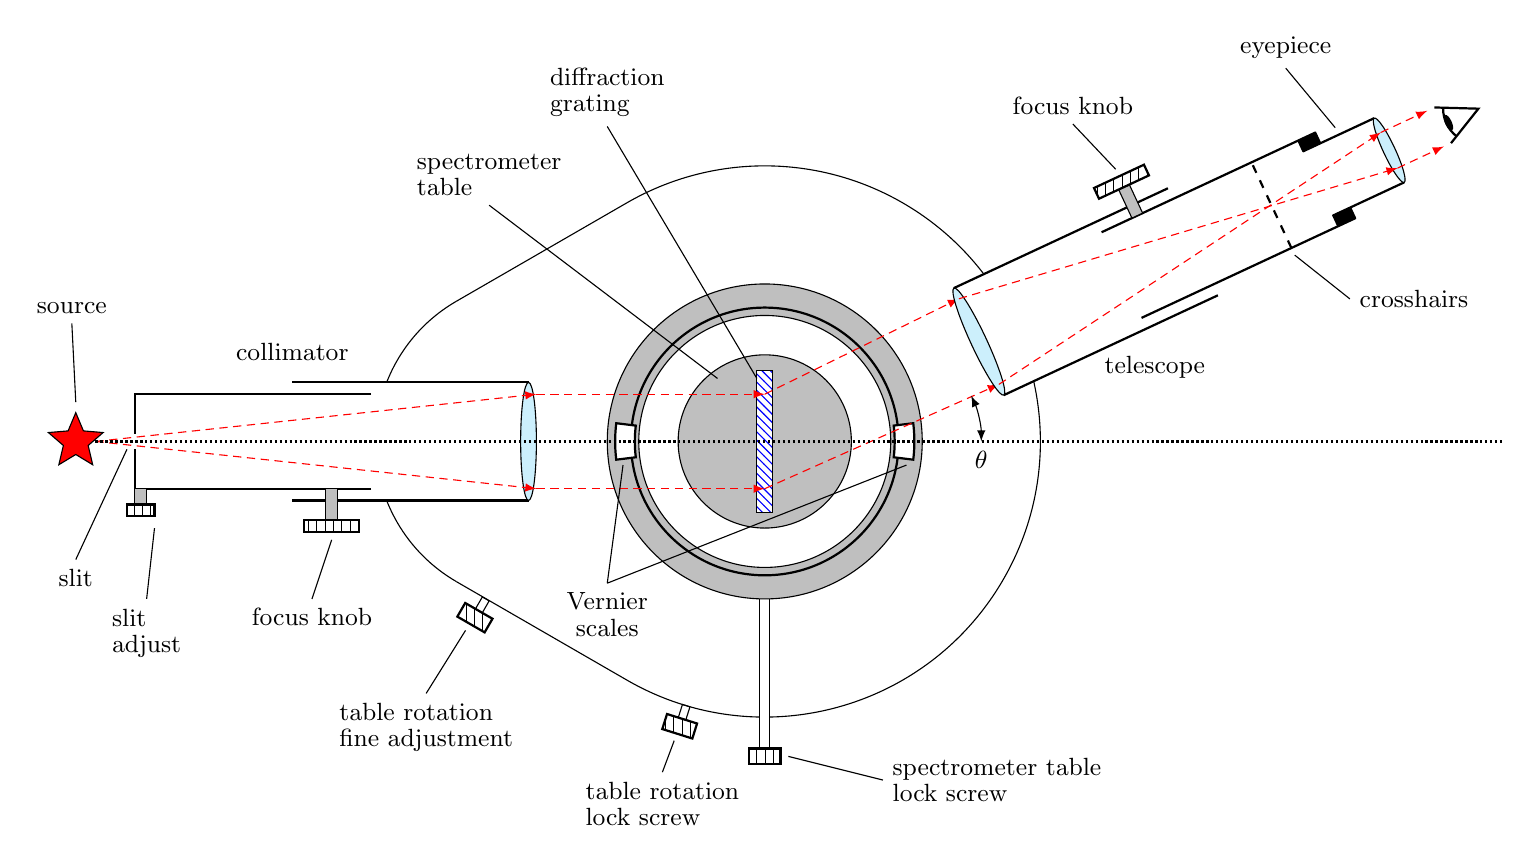
\begin{tikzpicture}
    % Table base
    \def\Ra{3.5};
    \def\Aa{120};
    \def\Ab{\Aa - 90};
    \def\Ac{180 - \Ab};
    \def\Rb{2.5}
    \draw ({\Ra*cos(\Aa)},{-\Ra*sin(\Aa)}) arc (-\Aa:\Aa:\Ra);
    \draw ({\Ra*cos(\Aa)},{-\Ra*sin(\Aa)}) -- ++({-\Rb*cos(\Ab)},{\Rb*sin(\Ab)});
    \draw ({\Ra*cos(\Aa)},{\Ra*sin(\Aa)}) -- ++({-\Rb*cos(\Ab)},{-\Rb*sin(\Ab)});
    \draw ({\Ra*cos(\Aa)-\Rb*cos(\Ab)},{\Ra*sin(\Aa)-\Rb*sin(\Ab)})
          arc (120:240:{\Ra-1.155*\Rb*sin(\Ab)});
    % Table base lock screw and adjustment screw
    \begin{scope}[rotate around={\Ac:(-3.5,-2.025)}]
        \draw[thick,pattern=vertical lines] (-3.75,-2.2) rectangle (-3.35,-2.4);
        \draw (-3.6,-2.2) rectangle (-3.5,-2.025);
    \end{scope}
    %
    \begin{scope}[rotate around={342.5:(-0.95,-3.37)}]
        \draw[thick,pattern=vertical lines] (-1.2,-3.545) rectangle (-0.8,-3.745);
        \draw (-1.05,-3.545) rectangle (-0.95,-3.37);
    \end{scope}
    % Spectrometer table adjustment screw
    \draw[fill=white] (-0.065,-1.1) rectangle (0.065,-3.9);
    \draw[thick, pattern=vertical lines] (-0.2,-3.9) rectangle (0.2,-4.1);
    % Turntable, grating, and vernier window
    \draw[fill=gray!50] (0,0) circle (2cm);
    \draw[thick] (0,0) circle (1.7cm);
    \draw[fill=white] (0,0) circle (1.6cm);
    \draw[fill=gray!50] (0,0) circle (1.1cm);
    \draw[fill=white] (-0.1,-0.9) rectangle (0.1,0.9);
    \draw[pattern=north west lines, pattern color=blue] (-0.1,-0.9) rectangle (0.1,0.9);
    \def\Rin{1.65};
    \def\Rout{1.9};
    \def\AngAStart{180 - 7};
    \def\AngAStop{180 + 7};
    \def\AngBStart{-7};
    \def\AngBStop{7};
    \filldraw[fill=white, draw=black, thick]
        (\AngAStart:\Rin)
        arc[radius=\Rin, start angle=\AngAStart, end angle=\AngAStop] --
        (\AngAStop:\Rout)
        arc[radius=\Rout, start angle=\AngAStop, end angle=\AngAStart] --
        cycle;
    \filldraw[fill=white, draw=black, thick]
        (\AngBStart:\Rin)
        arc[radius=\Rin, start angle=\AngBStart, end angle=\AngBStop] --
        (\AngBStop:\Rout)
        arc[radius=\Rout, start angle=\AngBStop, end angle=\AngBStart] --
        cycle;
    % Collimator
    \draw[color=white, fill=white] (-3,0.75) rectangle (-6,-0.75);
    \draw[thick] (-3,0.75) -- (-6,0.75);
    \draw[thick] (-3,-0.75) -- (-6,-0.75);
    \draw[fill=cyan!20] (-3,0) ellipse (0.1 cm and 0.75cm);
    \draw[thick] (-5,0.6) -- (-8,0.6) -- (-8,0.1);
    \draw[thick] (-5,-0.6) -- (-8,-0.6) -- (-8,-0.1);
    % Collimator and slit adjustment knobs
    \draw[fill=gray!50] (-5.425,-0.6) rectangle (-5.575,-1);
    \draw[thick,pattern=vertical lines] (-5.15,-1) rectangle (-5.85,-1.15);
    \draw[fill=gray!50] (-8,-0.6) rectangle (-7.85,-0.8);
    \draw[thick,pattern=vertical lines] (-8.1,-0.8) rectangle (-7.75,-0.95);
    % Source
    \node [star, star point height=2mm, minimum size=1mm, fill=red, draw] at (-8.75,0) {};
    % Rays from source to collimator lens
    \draw[-latex, densely dashed, red] (-8.5,0) -- (-2.9,0.6);
    \draw[-latex, densely dashed, red] (-8.5,0) -- (-2.9,-0.6);
    % Rays from collimator lens to grating
    \draw[-latex, densely dashed, red] (-2.9,0.6) -- (0,0.6);
    \draw[-latex, densely dashed, red] (-2.9,-0.6) -- (0,-0.6);
    % Rays from grating to telescope lens
    % Define a rotation angle.
    \def\RotAngle{25};
    \draw[-latex, densely dashed, red] (0,0.6) -- ({3*cos(\RotAngle)-0.6*sin(\RotAngle)},{3*sin(\RotAngle)+0.6*cos(\RotAngle)});
    \draw[-latex, densely dashed, red] (0,-0.6) -- ({3*cos(\RotAngle)+0.6*sin(\RotAngle)},{3*sin(\RotAngle)-0.6*cos(\RotAngle)});
    \begin{scope}[rotate around={\RotAngle:(0,0)}]
        % Telescope
        \draw[color=white, fill=white] (3,0.75) rectangle (6,-0.75);
        \draw[thick] (3,0.75) -- (6,0.75);
        \draw[thick] (3,-0.75) -- (6,-0.75);
        \draw[fill=cyan!20] (3,0) ellipse (0.1 cm and 0.75cm);
        \draw[thick] (5,0.6) -- (8,0.6);
        \draw[thick] (5,-0.6) -- (8,-0.6);
        \draw[thick, dashed] (7.1,-0.6) -- (7.1,0.6);
        \draw[thick] (7.75,0.45) -- (8.75,0.45);
        \draw[thick] (7.75,-0.45) -- (8.75,-0.45);
        \draw[fill=black] (7.75,0.45) rectangle (8,0.6);
        \draw[fill=black] (7.75,-0.45) rectangle (8,-0.6);
        \draw[fill=cyan!20] (8.75,0) ellipse (0.075 cm and 0.45cm);
        % Telescope adjustment knob
        \draw[fill=gray!50] (5.425,0.6) rectangle (5.575,1);
        \draw[thick,pattern=vertical lines] (5.15,1) rectangle (5.85,1.15);
        % Draw observer eyeball
        \draw[thick] (9.5,0.25) -- (10,0) -- (9.5,-0.25);
        \draw[thick] (9.6,-0.2) arc ({180+26.56}:155:0.45);
        \draw[fill=black] (9.58,0) ellipse (0.35mm and 1mm);
        % Rays from telescope lens to eyepiece lens
        \draw[-latex, densely dashed, red] (3,0.6) -- (8.75,-0.25);
        \draw[-latex, densely dashed, red] (3,-0.6) -- (8.75,0.25);
        \draw[-latex, densely dashed, red] (8.75,-0.25) -- (9.4,-0.25);
        \draw[-latex, densely dashed, red] (8.75,0.25) -- (9.4,0.25);
        %
        % Labels
        %
        \draw (5,-1) node[below] {\small telescope};
        \draw (5.25,2) node[above] {\small focus knob} -- (5.5,1.25);
        \draw (8,1.5) node[above] {\small eyepiece} -- (8.25,0.55);
        \draw (7.5,-1.5) node[right, align=left] {\small crosshairs} -- (7.1,-0.7);
    \end{scope}
    % Draw straight-through line
    \draw[densely dotted, thick] (-8.5,0) -- (9.4,0);
    %
    % Add some labels
    %
    \draw[latex-latex] (2.75,0) node[below] {\small $\theta$} arc (0:{\RotAngle}:1.375);
    \draw (-2,4) node[above, align=left] {\small diffraction\\[-0.25em] \small grating} -- (-0.1,0.8);
    \draw (-3.5,3) node[above, align=left] {\small spectrometer\\[-0.25em] \small table} -- (-0.6,0.8);
    \draw (-2,-1.8) node[below, align=center] {\small Vernier\\[-0.25em] \small scales} -- (-1.8,-0.3);
    \draw (-2,-1.8) -- (1.8,-0.3);
%    \draw (2,-1.5) node[right, align=left] {\small telescope\\[-0.25em] \small turntable} -- (1,-0.7);
    \draw (-6,0.9) node[above] {\small collimator};
    \draw (-5.75,-2) node[below] {\small focus knob} -- (-5.5,-1.25);
    \draw (-7.85,-2) node[below, align=left] {\small slit\\[-0.25em] \small adjust} -- (-7.75,-1.1);
    \draw (-8.75,-1.5) node[below] {\small slit} -- (-8.1,-0.1);
    \draw (-8.8,1.5) node[above] {\small source} -- (-8.75,0.5);
    \draw (-1.15,-3.8) -- (-1.3,-4.2) node[below, align=left] {\small table rotation\\[-0.25em] \small lock screw};
    \draw (-3.8,-2.4) -- (-4.3,-3.2) node[below, align=left] {\small table rotation\\[-0.25em] \small fine adjustment};
    \draw (0.3,-4) -- (1.5,-4.3) node[right, align=left] {\small spectrometer table\\[-0.25em] \small lock screw};
\end{tikzpicture}

% \end{document}
}
    \caption{Diagram of the spectrometer to be used in the lab.}
    \label{fig: spectrometer}
\end{figure}

The physical grating is situated on one side or face of a slab of glass. The grating holder in your setup (see Fig.~\ref{fig: spectrometer}) should specify the face upon which the grating has been placed. The grating will also be labeled with the number of grooves per mm. This number is approximate only, and the true grating separation must be measured.

In the first part of the lab, you will align your spectrometer so that the telescope and collimator are focused properly on the slit image, and the grating is perfectly perpendicular to the optical path. Next, you will calibrate the groove separation of your particular grating by using a
known wavelength of the sodium spectrum. Finally, you will measure the angles of some of the spectral lines of the Balmer series. These angles will be converted to wavelength using the calibration value you obtain for the grating.

\end{theory}

\begin{equipment}
\item lasers
\item sharks
\end{equipment}

\begin{experiment}
\subsection*{Measuring Angles Precisely with a Vernier Scale}

To precisely measure the wavelengths of the hydrogen spectrum, we will need to record angles to the nearest arcminute (\qty{1}{\arcminute}=1/60\qty{}{\degree}). 
To do this, we use a vernier scale comprising a degree scale on the spectrometer table and a secondary scale accurate to \qty{1}{\arcminute}.
There are two windows on the table platform with degree and vernier scales, as shown in Fig.~\ref{fig: spectrometer}.

\begin{figure}
    \centering
    
\includegraphics[width=0.6\linewidth]{Lab 14: The Atomic Spectrum of Hydrogen/vernier-scale.png}
    \caption{The vernier scale and degree plate on the spectrometer. Credit: PASCO Scientific.}
    \label{fig: vernier scale}
\end{figure}

Figure~\ref{fig: vernier scale} shows an example angle reading on the scale. To read the angle, first find where the zero point of the vernier scale aligns with the degree plate and record the value. If the zero point of the vernier scale is between two lines on the degree scale, use the smaller degree value. In Fig.~\ref{fig: vernier scale}, the zero point on the vernier scale is between the \qty{155}{\degree} and \qty{155}{\degree}\qty{30}{\arcminute} marks on the degree plate, so the recorded value is \qty{155}{\degree}.

Next, use the magnifying glass to find the line on the vernier scale that aligns most closely with any line on the degree scale. In Fig.~\ref{fig: vernier scale}, this is the line corresponding to a measurement of \qty{15}{\arcminute}. Add this value to the course reading recorded above to get the correct measurement to within 1 minute of arc:
\[
    \qty{155}{\degree} + \qty{15}{\arcminute} = \qty{155}{\degree}\qty{15}{\arcminute} = \qty{150.25}{\degree}.
\]

\subsection*{Alignment of the Spectrometer}

The spectrometer needs to be aligned (see Fig.~\ref{fig: aligned spectrometer}) to ensure accurate measurements of the sodium spectral calibration lines and the hydrogen spectral lines. Loosening the locking screw right below the telescope (not shown in Fig.~\ref{fig: spectrometer} allows it to rotate. Loosening the lock screw on the long stalk below the spectrometer table (shown in Fig.~\ref{fig: spectrometer}) allows the grating to rotate, and if you loosen the table rotation lock screw, you will allow the platform to rotate. If you rotate the platform, then the angles visible in the window on the platform will change. Learn how to keep a careful track of these changes.

\subsubsection*{Procedure}

\begin{enumerate}
    \item Turn on the Na lamp. It needs a few minutes to warm up. You will know it is ready when the emitted light has a warm yellow glow. Place the lamp in front of the slit, as shown in Fig.~\ref{fig: aligned spectrometer}, and center it by eye as best you can.
    %
    \item Familiarize yourself with all of the controls on the spectrometer. Learn the effect of loosening and tightening each knob as described above. By mastering the operation of the spectrometer \textsl{now}, you will save yourself time and frustration if you were to loosen or tighten something incorrectly \textsl{later}.
    %
    \item Rotate the telescope so that it points at a far wall with no obstruction (i.e., it does not look at the slit.) Focus the telescope at infinity -- for instance, use an object on a faraway wall to focus.

    \begin{figure}[ht]
        \centering
        \scalebox{0.85}{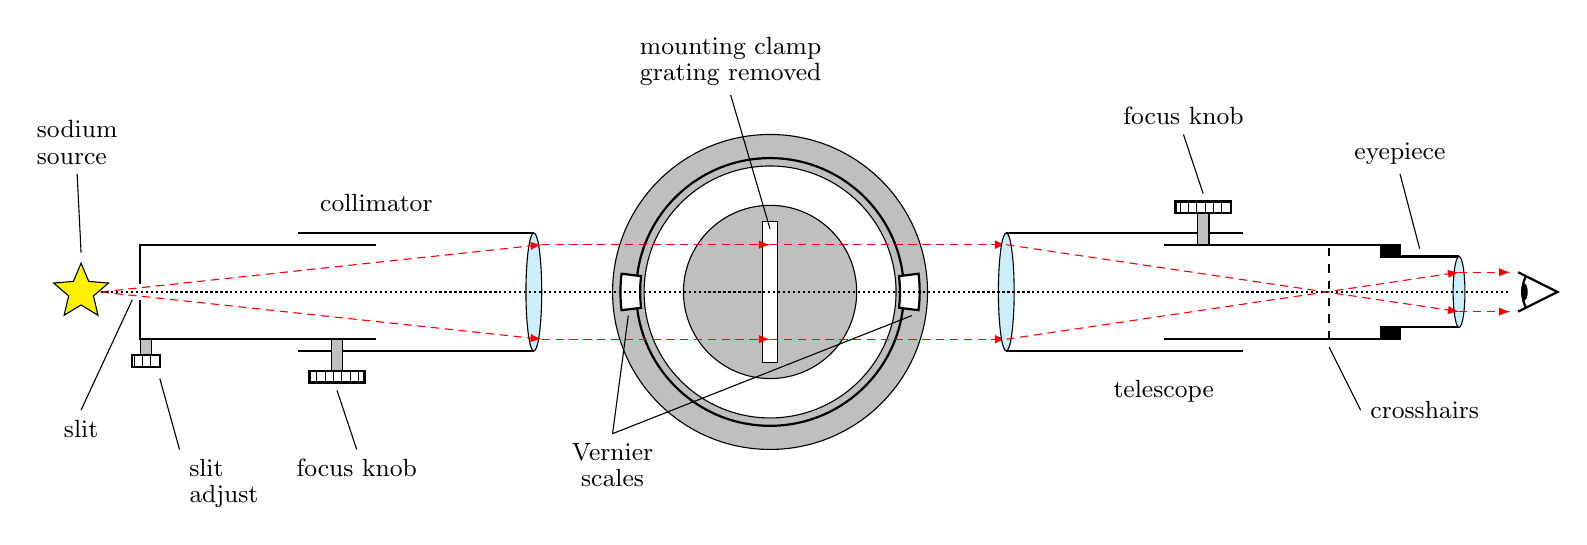
\begin{tikzpicture}
    % Turntable, grating, and vernier windows
    \draw[fill=gray!50] (0,0) circle (2cm);
    \draw[thick] (0,0) circle (1.7cm);
    \draw[fill=white] (0,0) circle (1.6cm);
    \draw[fill=gray!50] (0,0) circle (1.1cm);
    \draw[fill=white] (-0.1,-0.9) rectangle (0.1,0.9);
    % \draw[pattern=north west lines, pattern color=blue] (-0.1,-0.9) rectangle (0.1,0.9);
    \def\Rin{1.65};
    \def\Rout{1.9};
    \def\AngAStart{180 - 7};
    \def\AngAStop{180 + 7};
    \def\AngBStart{-7};
    \def\AngBStop{7};
    \filldraw[fill=white, draw=black, thick]
        (\AngAStart:\Rin)
        arc[radius=\Rin, start angle=\AngAStart, end angle=\AngAStop] --
        (\AngAStop:\Rout)
        arc[radius=\Rout, start angle=\AngAStop, end angle=\AngAStart] --
        cycle;
    \filldraw[fill=white, draw=black, thick]
        (\AngBStart:\Rin)
        arc[radius=\Rin, start angle=\AngBStart, end angle=\AngBStop] --
        (\AngBStop:\Rout)
        arc[radius=\Rout, start angle=\AngBStop, end angle=\AngBStart] --
        cycle;
    % Collimator
    \draw[thick] (-3,0.75) -- (-6,0.75);
    \draw[thick] (-3,-0.75) -- (-6,-0.75);
    \draw[fill=cyan!20] (-3,0) ellipse (0.1 cm and 0.75cm);
    \draw[thick] (-5,0.6) -- (-8,0.6) -- (-8,0.1);
    \draw[thick] (-5,-0.6) -- (-8,-0.6) -- (-8,-0.1);
    % Collimator and slit adjustment knobs
    \draw[fill=gray!50] (-5.425,-0.6) rectangle (-5.575,-1);
    \draw[thick,pattern=vertical lines] (-5.15,-1) rectangle (-5.85,-1.15);
    \draw[fill=gray!50] (-8,-0.6) rectangle (-7.85,-0.8);
    \draw[thick,pattern=vertical lines] (-8.1,-0.8) rectangle (-7.75,-0.95);
    % Source
    \node [star, star point height=2mm, minimum size=1mm, fill=yellow, draw] at (-8.75,0) {};
    % Rays from source to collimator lens
    \draw[-latex, densely dashed, red] (-8.5,0) -- (-2.9,0.6);
    \draw[-latex, densely dashed, red] (-8.5,0) -- (-2.9,-0.6);
    % Rays from collimator lens to grating
    \draw[-latex, densely dashed, red] (-2.9,0.6) -- (0,0.6);
    \draw[-latex, densely dashed, red] (-2.9,-0.6) -- (0,-0.6);
    % Rays from grating to telescope lens
    % Define a rotation angle.
    \def\RotAngle{0};
    \draw[-latex, densely dashed, red] (0,0.6) -- ({3*cos(\RotAngle)-0.6*sin(\RotAngle)},{3*sin(\RotAngle)+0.6*cos(\RotAngle)});
    \draw[-latex, densely dashed, red] (0,-0.6) -- ({3*cos(\RotAngle)+0.6*sin(\RotAngle)},{3*sin(\RotAngle)-0.6*cos(\RotAngle)});
    \begin{scope}[rotate around={\RotAngle:(0,0)}]
        % Telescope
        \draw[thick] (3,0.75) -- (6,0.75);
        \draw[thick] (3,-0.75) -- (6,-0.75);
        \draw[fill=cyan!20] (3,0) ellipse (0.1 cm and 0.75cm);
        \draw[thick] (5,0.6) -- (8,0.6);
        \draw[thick] (5,-0.6) -- (8,-0.6);
        \draw[thick, dashed] (7.1,-0.6) -- (7.1,0.6);
        \draw[thick] (7.75,0.45) -- (8.75,0.45);
        \draw[thick] (7.75,-0.45) -- (8.75,-0.45);
        \draw[fill=black] (7.75,0.45) rectangle (8,0.6);
        \draw[fill=black] (7.75,-0.45) rectangle (8,-0.6);
        \draw[fill=cyan!20] (8.75,0) ellipse (0.075 cm and 0.45cm);
        % Telescope adjustment knob
        \draw[fill=gray!50] (5.425,0.6) rectangle (5.575,1);
        \draw[thick,pattern=vertical lines] (5.15,1) rectangle (5.85,1.15);
        % Draw observer eyeball
        \draw[thick] (9.5,0.25) -- (10,0) -- (9.5,-0.25);
        \draw[thick] (9.6,-0.2) arc ({180+26.56}:155:0.45);
        \draw[fill=black] (9.58,0) ellipse (0.35mm and 1mm);
        % Rays from telescope lens to eyepiece lens
        \draw[-latex, densely dashed, red] (3,0.6) -- (8.75,-0.25);
        \draw[-latex, densely dashed, red] (3,-0.6) -- (8.75,0.25);
        \draw[-latex, densely dashed, red] (8.75,-0.25) -- (9.4,-0.25);
        \draw[-latex, densely dashed, red] (8.75,0.25) -- (9.4,0.25);
        %
        % Labels
        %
        \draw (5,-1) node[below] {\small telescope};
        \draw (5.25,2) node[above] {\small focus knob} -- (5.5,1.25);
        \draw (8,1.5) node[above] {\small eyepiece} -- (8.25,0.55);
        \draw (7.5,-1.5) node[right, align=left] {\small crosshairs} -- (7.1,-0.7);
    \end{scope}
    % Draw straight-through line 
    \draw[densely dotted, thick] (-8.5,0) -- (9.4,0);
    %
    % Add some labels
    %
    % \draw[latex-latex] (2.75,0) node[below] {\small $\theta$} arc (0:{\RotAngle}:1.375);
    \draw (-0.5,2.5) node[above, align=left] {\small mounting clamp\\[-0.25em] \small grating removed} -- (0,0.8);
    \draw (-2,-1.8) node[below, align=center] {\small Vernier\\[-0.25em] \small scales} -- (-1.8,-0.3);
    \draw (-2,-1.8) -- (1.8,-0.3);
    % \draw (2,-1.5) node[right, align=left] {\small telescope\\ \small turntable} -- (1,-0.7);
    \draw (-5,0.9) node[above] {\small collimator};
    \draw (-5.25,-2) node[below] {\small focus knob} -- (-5.5,-1.25);
    \draw (-7.5,-2) node[below right, align=left] {\small slit\\[-0.25em] \small adjust} -- (-7.75,-1.1);
    \draw (-8.75,-1.5) node[below] {\small slit} -- (-8.1,-0.1);
    \draw (-8.8,1.5) node[above, align=left] {\small sodium\\[-0.25em] \small source} -- (-8.75,0.5);
\end{tikzpicture}}
        \caption{Aligned orientation of the spectrometer to be used in alignment steps \ref{step: align 1}, \ref{step: align 2}, and \ref{step: align 3}.}
        \label{fig: aligned spectrometer}
    \end{figure}

    %
    \item \label{step: align 1} With the grating removed, align the telescope with the collimator/slit component as shown in Fig.~\ref{fig: aligned spectrometer}. Adjust the slit and collimator to produce a sharp, narrow image of the source (slit). Make sure you DO NOT REFOCUS THE TELESCOPE.
    %
    \item \label{step: align 2} Center the crosshairs on the image of the slit.
    %
    \item \label{step: align 3} Record the angle displayed in the window in Data Table~\ref{data: spectrometer setup} in the Postlab exercises; this is your initial zero angle $\theta_{0,i}$. There are two vernier windows on the spectrometer platform; be sure to use the same window for the entire lab.
    %
    \item \label{step: rotate 1} Replace the grating and ensure the grating lines or ``rules'' are perpendicular to the platform; i.e., they should point toward the ceiling. The grating face should face the slit side of the spectrometer. Record the number of lines/mm of your grating in Data Table~\ref{data: spectrometer setup} of the Postlab exercises. If you have the option, choose the 600~grooves/mm grating. With the grating fixed in place, rotate the telescope exactly \qty{90}{\degree} as shown in Fig.~\ref{fig: spectrometer rotated} and then fix the telescope in place.

    \begin{figure}[ht]
        \centering
        \scalebox{0.5}{\input{Lab 14: The Atomic Spectrum of Hydrogen/spectrometer-90-deg.tex}}
        \hfill
        \scalebox{0.5}{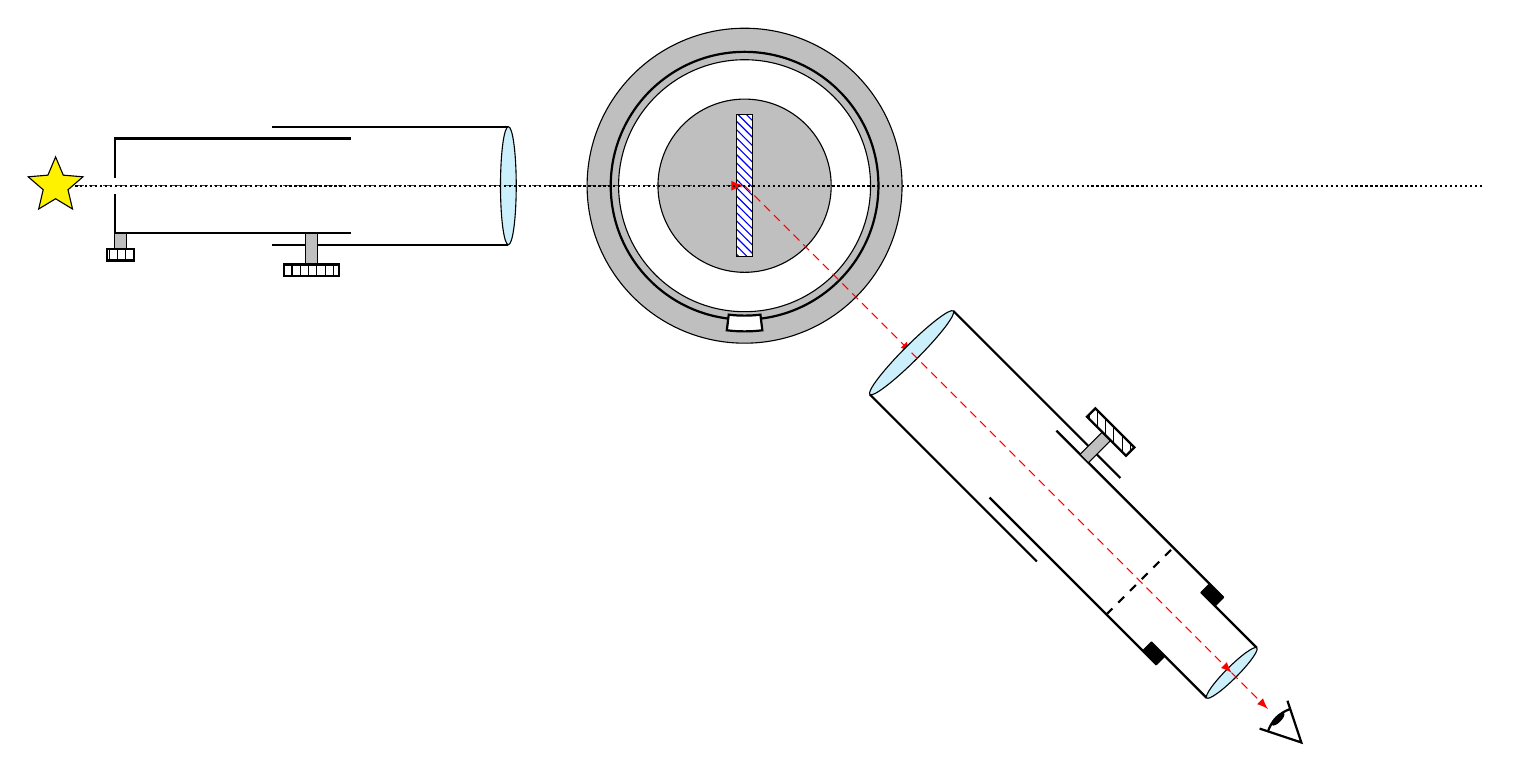
\begin{tikzpicture}
    % Turntable, grating, and vernier window
    \draw[fill=gray!50] (0,0) circle (2cm);
    \draw[thick] (0,0) circle (1.7cm);
    \draw[fill=white] (0,0) circle (1.6cm);
    \draw[fill=gray!50] (0,0) circle (1.1cm);
    \draw[fill=white] (-0.1,-0.9) rectangle (0.1,0.9);
    \draw[pattern=north west lines, pattern color=blue] (-0.1,-0.9) rectangle (0.1,0.9);
    \def\Rin{1.65};
    \def\Rout{1.85};
    \def\StartAngle{263};
    \def\StopAngle{277};
    \filldraw[fill=white, draw=black, thick]
        (\StartAngle:\Rin)
        arc[radius=\Rin, start angle=\StartAngle, end angle=\StopAngle] --
        (\StopAngle:\Rout)
        arc[radius=\Rout, start angle=\StopAngle, end angle=\StartAngle] --
        cycle;
    % Collimator
    \draw[thick] (-3,0.75) -- (-6,0.75);
    \draw[thick] (-3,-0.75) -- (-6,-0.75);
    \draw[fill=cyan!20] (-3,0) ellipse (0.1 cm and 0.75cm);
    \draw[thick] (-5,0.6) -- (-8,0.6) -- (-8,0.1);
    \draw[thick] (-5,-0.6) -- (-8,-0.6) -- (-8,-0.1);
    % Collimator and slit adjustment knobs
    \draw[fill=gray!50] (-5.425,-0.6) rectangle (-5.575,-1);
    \draw[thick,pattern=vertical lines] (-5.15,-1) rectangle (-5.85,-1.15);
    \draw[fill=gray!50] (-8,-0.6) rectangle (-7.85,-0.8);
    \draw[thick,pattern=vertical lines] (-8.1,-0.8) rectangle (-7.75,-0.95);
    % Source
    \node [star, star point height=2mm, minimum size=1mm, fill=yellow, draw] at (-8.75,0) {};
    % Rays from source to grating and to telescope
    \draw[-Latex, densely dashed, red] (-8.5,0) -- (0,0);
    % Rays from grating to telescope lens
    % Define a rotation angle.
    \def\RotAngle{-45};
    \draw[-latex, densely dashed, red] (0,0) -- ({3*cos(\RotAngle)-0*sin(\RotAngle)},{3*sin(\RotAngle)+0*cos(\RotAngle)});
    \begin{scope}[rotate around={\RotAngle:(0,0)}]
        % Telescope
        \draw[thick] (3,0.75) -- (6,0.75);
        \draw[thick] (3,-0.75) -- (6,-0.75);
        \draw[fill=cyan!20] (3,0) ellipse (0.1 cm and 0.75cm);
        \draw[thick] (5,0.6) -- (8,0.6);
        \draw[thick] (5,-0.6) -- (8,-0.6);
        \draw[thick, dashed] (7.1,-0.6) -- (7.1,0.6);
        \draw[thick] (7.75,0.45) -- (8.75,0.45);
        \draw[thick] (7.75,-0.45) -- (8.75,-0.45);
        \draw[fill=black] (7.75,0.45) rectangle (8,0.6);
        \draw[fill=black] (7.75,-0.45) rectangle (8,-0.6);
        \draw[fill=cyan!20] (8.75,0) ellipse (0.075 cm and 0.45cm);
        % Telescope adjustment knob
        \draw[fill=gray!50] (5.425,0.6) rectangle (5.575,1);
        \draw[thick,pattern=vertical lines] (5.15,1) rectangle (5.85,1.15);
        % Draw observer eyeball
        \draw[thick] (9.5,0.25) -- (10,0) -- (9.5,-0.25);
        \draw[thick] (9.6,-0.2) arc ({180+26.56}:155:0.45);
        \draw[fill=black] (9.58,0) ellipse (0.35mm and 1mm);
        % Rays from telescope lens to eyepiece lens
        \draw[-latex, densely dashed, red] (3,0) -- (8.75,0);
        \draw[-latex, densely dashed, red] (8.75,0) -- (9.4,0);
    \end{scope}
    % Draw straight-through line 
    \draw[densely dotted, thick] (-8.5,0) -- (9.4,0);
\end{tikzpicture}}
        \caption{Left: \qty{90}{\degree} orientation of the spectrometer for parts \ref{step: rotate 1} and \ref{step: rotate 2} of the alignment procedure. Note the \qty{45}{\degree} angle of the grating. Right: \qty{135}{\degree} orientation of the spectrometer for step \ref{step: rotate 3} of the alignment procedure. Note the perpendicular alignment of the grating.}
        \label{fig: spectrometer rotated}
    \end{figure}

    \item \label{step: rotate 2} Rotate the grating until the slit image of the Na light source is centered on the crosshairs. Use the zero-order spectrum, i.e., the reflection of the light bulb itself, not a spectral line. The incident angle of the light is now certain to be \qty{45}{\degree}.

    \item Fix the grating in place, making sure that the crosshairs stay centered on the light.

    \item \label{step: rotate 3} Turn the telescope back \qty{90}{\degree} to its original position, as in Fig.~\ref{fig: aligned spectrometer} and then rotate \textbf{the platform} by \qty{135}{\degree}, so that the light from the source is normal to the grating (see Fig.~\ref{fig: spectrometer rotated}). The grating face is now facing the telescope side of the spectrometer so that the light from the source passes through the grating last of all. The crosshairs should be centered on the slit. Record the final zero angle, $\theta_{0,f}$, if different from $\theta_{0,i}$. You will be using this final zero angle in all subsequent measurements with the spectrometer, as you will be subtracting it from your measured values of angle for all spectral lines.
    
\end{enumerate}

\subsection*{Calibration of the Diffraction Grating}

In this part of the experiment, you will determine your grating separation by measuring the angle of the sodium D-lines of the sodium excitation spectrum. The sodium D-lines are a pair of yellow spectral lines, called a ``doublet,'' that have wavelengths of \qty{589.0}{\nano\meter} and \qty{589.6}{\nano\meter}, respectively. You should be able to resolve the doublet, and thus measure a distinct angle for each spectral line, with a little care. It will also be helpful if you are using a 600~groove/mm grating and minimize the width of the slit using the slit adjustment
thumbscrew. If you cannot resolve the doublet, measure the average angle at which the yellow line appears and then average the two wavelength values given above.

\subsubsection*{Procedure}

\begin{enumerate}
    \item Start with the telescope set to the final zero angle position $\theta_{0,f}$. Move the telescope to the left until you come across the first pair of yellow lines. This angle will be the first-order spectrum value ($m=1$). Record this angle (or angles if you can resolve the doublet) in Data Table~\ref{data: sodium calibration}. Now measure the first-order position(s) in the opposite direction (the right side). Record the angle(s) in Data Table~\ref{data: sodium calibration}. You should now be able to determine the grating spacing of your particular grating, using eq.~\ref{eq: grating equation} and the average first-order angle(s) of the sodium line(s). You do not need to measure the second-order lines ($m=2$).
    %
    \item In filling out \textbf{Table 14.2}, the Measured Angle is the number read from the vernier scale, the Difference Angle is the positive angle difference of the $\theta_{0,f}$ and the Measured Angle, and the Average Angle is the average of the two Difference Angles. Average Angle is the value you use to calculate the grating separation according to eq.~\ref{eq: grating equation}.
\end{enumerate}

\begin{figure}[ht]
    \centering
    \scalebox{0.85}{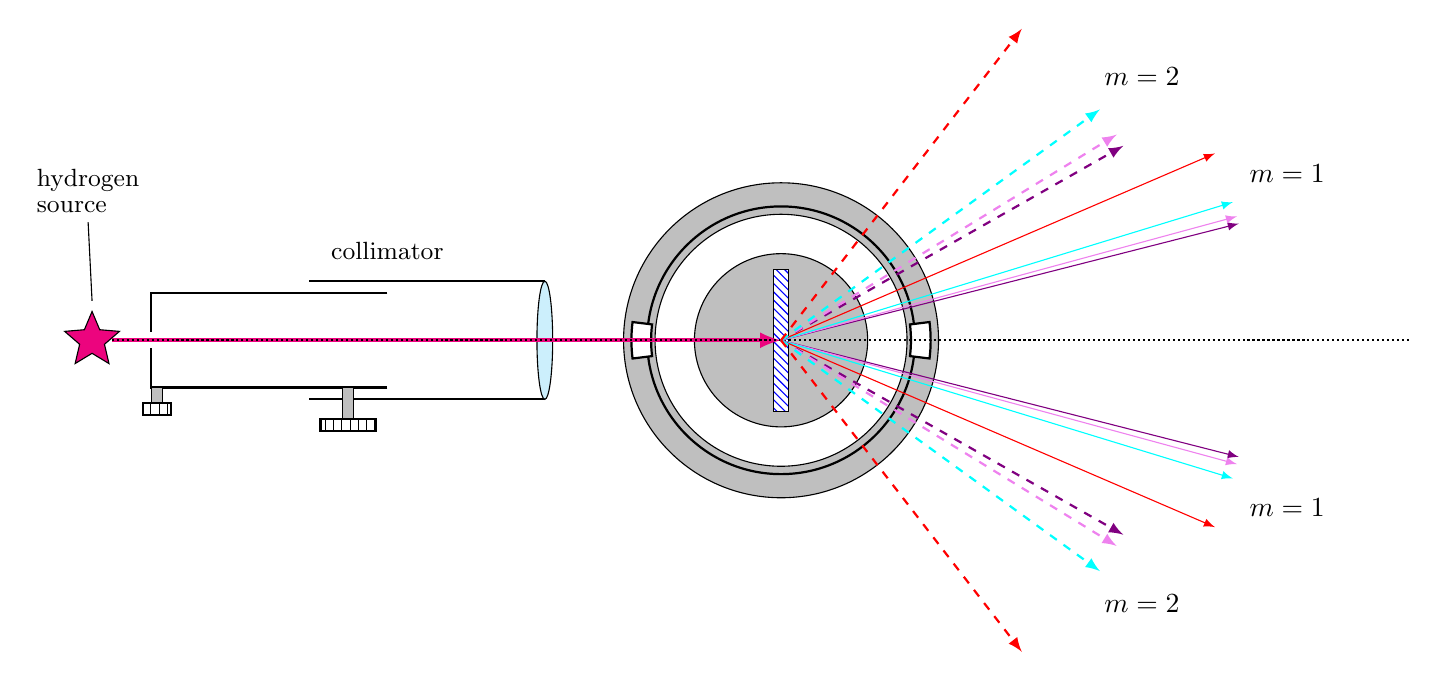
\begin{tikzpicture}
    % Turntable, grating, and vernier window
    \draw[fill=gray!50] (0,0) circle (2cm);
    \draw[thick] (0,0) circle (1.7cm);
    \draw[fill=white] (0,0) circle (1.6cm);
    \draw[fill=gray!50] (0,0) circle (1.1cm);
    \draw[fill=white] (-0.1,-0.9) rectangle (0.1,0.9);
    \draw[pattern=north west lines, pattern color=blue] (-0.1,-0.9) rectangle (0.1,0.9);
    \def\Rin{1.65};
    \def\Rout{1.9};
    \def\AngAStart{180 - 7};
    \def\AngAStop{180 + 7};
    \def\AngBStart{-7};
    \def\AngBStop{7};
    \filldraw[fill=white, draw=black, thick]
        (\AngAStart:\Rin)
        arc[radius=\Rin, start angle=\AngAStart, end angle=\AngAStop] --
        (\AngAStop:\Rout)
        arc[radius=\Rout, start angle=\AngAStop, end angle=\AngAStart] --
        cycle;
    \filldraw[fill=white, draw=black, thick]
        (\AngBStart:\Rin)
        arc[radius=\Rin, start angle=\AngBStart, end angle=\AngBStop] --
        (\AngBStop:\Rout)
        arc[radius=\Rout, start angle=\AngBStop, end angle=\AngBStart] --
        cycle;
    % Collimator
    \draw[color=white, fill=white] (-3,0.75) rectangle (-6,-0.75);
    \draw[thick] (-3,0.75) -- (-6,0.75);
    \draw[thick] (-3,-0.75) -- (-6,-0.75);
    \draw[fill=cyan!20] (-3,0) ellipse (0.1 cm and 0.75cm);
    \draw[thick] (-5,0.6) -- (-8,0.6) -- (-8,0.1);
    \draw[thick] (-5,-0.6) -- (-8,-0.6) -- (-8,-0.1);
    % Collimator and slit adjustment knobs
    \draw[fill=gray!50] (-5.425,-0.6) rectangle (-5.575,-1);
    \draw[thick,pattern=vertical lines] (-5.15,-1) rectangle (-5.85,-1.15);
    \draw[fill=gray!50] (-8,-0.6) rectangle (-7.85,-0.8);
    \draw[thick,pattern=vertical lines] (-8.1,-0.8) rectangle (-7.75,-0.95);
    % Source
    \node [star, star point height=2mm, minimum size=1mm, fill=RubineRed, draw] at (-8.75,0) {};
    % Rays from source to collimator lens
    \draw[ultra thick, -latex, RubineRed] (-8.5,0) -- (0,0);
    % Draw straight-through line
    \draw[densely dotted, thick] (-8.5,0) -- (8,0);
    %
    % Draw Balmer lines (n=1)
    %
    \foreach \ang/\wlcolor in {{14.3/Purple}, {15.2/Violet}, {17.0/Cyan}, {23.3/Red}} {
      \draw[-latex, color=\wlcolor] (0,0) -- ({6*cos(\ang)}, {6*sin(\ang)});
      \draw[-latex, color=\wlcolor] (0,0) -- ({6*cos(-\ang)}, {6*sin(-\ang)});
    }
    \draw ({6.2*cos(20)}, {6.2*sin(20)}) node[right] {$m=1$};
    \draw ({6.2*cos(340)}, {6.2*sin(340)}) node[right] {$m=1$};
    %
    % Draw Balmer lines (n=2)
    %
    \foreach \ang/\wlcolor in {{29.6/Purple}, {31.5/Violet}, {35.9/Cyan}, {52.3/Red}} {
      \draw[thick, -latex, color=\wlcolor, dashed] (0,0) -- ({5*cos(\ang)}, {5*sin(\ang)});
      \draw[thick, -latex, color=\wlcolor, dashed] (0,0) -- ({5*cos(-\ang)}, {5*sin(-\ang)});
    }
    \draw ({5.2*cos(40)}, {5.2*sin(40)}) node[right] {$m=2$};
    \draw ({5.2*cos(320)}, {5.2*sin(320)}) node[right] {$m=2$};
    %
    % Add some labels
    %
    \draw (-8.8,1.5) node[above, align=left] {\small hydrogen\\[-0.25em] \small source} -- (-8.75,0.5);
    \draw (-5,0.9) node[above] {\small collimator};
\end{tikzpicture}}
    \caption{Angles and diffraction orders of visible Balmer lines. Note that you may only be able to see three lines per order, not four.}
    \label{fig: balmer lines}
\end{figure}

\subsection*{The Balmer Series of Hydrogen}

Now you should be able to accurately measure the Balmer series for atomic hydrogen. 
You should be able to measure the first (solid) and second (dashed) orders for three Balmer lines: a red line (H$\alpha$), a cyan line (H$\beta$), and a blue line (H$\gamma$). 
You may also be able to resolve a violet line (H$\delta$). 
See Fig.~\ref{fig: balmer lines} for a picture of the relationship between the first ($m=1$) and second ($m=2$) orders.

\subsubsection*{Procedure}

\begin{enumerate}
    \item Replace the sodium lamp with the hydrogen lamp. 
    Make sure that the center of the hydrogen bulb aligns well with the spectrometer slit to maximize the intensity of the spectral lines. 
    You will need to protect your line of sight from all stray light to clearly see and measure the violet lines. 
    It may be helpful to carefully drape black cloth around your hydrogen lamp or over your spectrometer to prevent stray light from entering the spectrometer or from interfering with your ability to view the spectrum.
    %
    \item Record the angles at which each spectral line appears. You should measure both first and second orders on both the left and right sides of the zero angle of the red, cyan, and blue lines, for a total of 12 measurements. Record your data in Data Table~\ref{data: balmer data}.
\end{enumerate}

\end{experiment}

\end{labsection}

% POSTLAB SECTION
\begin{postlab}

    \fullwidth{\subsection*{Spectrometer Alignment and Calibration (\pointsinrange{calibration} points)}}
    \begingradingrange{calibration}

    \question[3] Fill in your zero angles and the grooves/mm written on the grating.

    \begin{center}
        \renewcommand{\arraystretch}{1.5}
        \captionsetup{font=normalsize}
        \captionof{data table}{Zero angles and diffraction grating size used in the spectrometer. \label{data: spectrometer setup}}
        \begin{tabular}{lrp{2cm}l}
        \hline
        \textbf{Quantity} & & \textbf{Value} &
        \\
        Initial zero angle: & $\theta_{i,0}=$ & &
        \\
        \cline{3-3}
        Final zero angle:   & $\theta_{0,f}=$ & &
        \\
        \cline{3-3}
        Grating dimension:  & $d=$ & & grooves/mm
        \\
        \cline{3-3}
        \end{tabular}
    \end{center}

    Next, fill in the calibration data from the sodium D-lines:

    \begin{center}
        \renewcommand{\arraystretch}{2}
        \captionsetup{font=normalsize}
        \captionof{data table}{Calibration data from sodium D-lines. \label{data: sodium calibration}}
        \begin{tabular}{|l|>{\centering\arraybackslash}p{1.8cm}|>{\centering\arraybackslash}p{1.8cm}|>{\centering\arraybackslash}p{1.8cm}|>{\centering\arraybackslash}p{1.8cm}|>{\centering\arraybackslash}p{2cm}|>{\centering\arraybackslash}p{2cm}|}
        \hline
        \rowcolor{gray!20}
        Spectral Line & Measured Angle & Difference Angle & Wavelength (nm) & Order $m$ & Grating sep. $d$ (nm) & $\overline{d}$ (nm)    \\
        \hline
        Left, Line 1  &                &                  &                 &           &                             & \multirow{4}{*}{} \\
        \cline{1-6}
        Right, Line 1 &                &                  &                 &           &                             &                   \\
        \cline{1-6}
        Left, Line 2  &                &                  &                 &           &                             &                   \\
        \cline{1-6}
        Right, Line 2 &                &                  &                 &           &                             &             
        \\
        \hline
        \end{tabular}
    \end{center}

    \filbreak
    \question[1] Show an example calculation of how you determined the grating spacing, $d$, using data from Data Table~\ref{data: sodium calibration}. Calculate an average value for $d$.
    %
    \begin{solution}[3cm]
        
    \end{solution}

    \filbreak
    \question[1] Calculate the uncertainty in grating separation, $\Delta d$, using the standard deviation of your two (or four) values for $d$.
    %
    \begin{solution}[2cm]
        
    \end{solution}

    \endgradingrange{calibration}

    \fullwidth{\subsection*{The Balmer Series (\pointsinrange{balmerdata} points)}}

    \begingradingrange{balmerdata}

    \filbreak
    \question[2] Fill in the table with your measurements of the Balmer lines.

    \begin{center}
        \renewcommand{\arraystretch}{2}
        \captionsetup{font=normalsize}
        \captionof{data table}{Balmer series measurements. \label{data: balmer data}}
        \begin{tabular}{|p{2cm}|c|>{\centering\arraybackslash}p{1.8cm}|>{\centering\arraybackslash}p{1.8cm}|>{\centering\arraybackslash}p{1.8cm}|>{\centering\arraybackslash}p{0.8cm}|>{\centering\arraybackslash}p{1.8cm}|>{\centering\arraybackslash}p{2cm}|}
            \hline
            \rowcolor{gray!20}
            Spectral Line & Order & Measured Angle & Difference Angle & Average Angle     & $m$               & Wavelength (nm)   & \textbf{Average Wavelength (nm)} \\
            \hline
            Red, Right    & 1st   &                &                  & \multirow{2}{*}{} & \multirow{2}{*}{} & \multirow{2}{*}{} & \multirow{4}{*}{}                \\
            \cline{1-4}
            Red, Left     & 1st   &                &                  &                   &                   &                   &                                  \\
            \cline{1-7}
            Red, Right    & 2nd   &                &                  & \multirow{2}{*}{} & \multirow{2}{*}{} & \multirow{2}{*}{} &                                  \\
            \cline{1-4}
            Red, Left     & 2nd   &                &                  &                   &                   &                   &                                  \\
            \hline
            Cyan, Right   & 1st   &                &                  & \multirow{2}{*}{} & \multirow{2}{*}{} & \multirow{2}{*}{} & \multirow{4}{*}{}                \\
            \cline{1-4}
            Cyan, Left    & 1st   &                &                  &                   &                   &                   &                                  \\
            \cline{1-7}
            Cyan, Right   & 2nd   &                &                  & \multirow{2}{*}{} & \multirow{2}{*}{} & \multirow{2}{*}{} &                                  \\
            \cline{1-4}
            Cyan, Left    & 2nd   &                &                  &                   &                   &                   &                                  \\
            \hline
            Blue, Right   & 1st   &                &                  & \multirow{2}{*}{} & \multirow{2}{*}{} & \multirow{2}{*}{} & \multirow{4}{*}{}                \\
            \cline{1-4}
            Blue, Left    & 1st   &                &                  &                   &                   &                   &                                  \\
            \cline{1-7}
            Blue, Right   & 2nd   &                &                  & \multirow{2}{*}{} & \multirow{2}{*}{} & \multirow{2}{*}{} &                                  \\
            \cline{1-4}
            Blue, Left    & 2nd   &                &                  &                   &                   &                   &                                 \\
            \hline
            \end{tabular}
    \end{center}

    \filbreak
    \question[1] Show the calculation for how you found the wavelength of the first-order blue line.
    %
    \begin{solution}[3cm]
        
    \end{solution}

    \filbreak
    \question[1] Show the calculation for how you found the wavelength of the second-order red line.
    %
    \begin{solution}[3cm]
        
    \end{solution}

    \filbreak
    \question[2] Calculate the uncertainty in wavelength $\Delta\lambda$ for the first-order cyan line using error propagation. Use the uncertainty in the grating separation that you determined earlier, and estimate a value for the uncertainty $\Delta\theta$, which you must convert to radians. Using the average angle $\theta$ when computing $\tan{\theta}$ in the expression below, compute $\Delta\lambda$:
    %
    \begin{equation}\label{eq: wavelenght uncertainty}
        \left(\frac{\Delta\lambda}{\lambda}\right)^2 = \left(\frac{\Delta d}{d}\right)^2 + \left(\frac{\Delta\theta}{\tan{\theta}}\right)^2.
    \end{equation}
    %
    \begin{solution}[6cm]
        
    \end{solution}

    \filbreak
    \question[1] Show the calculation for the theoretical Balmer wavelength for $n=3$ using Table~\ref{tab: hydrogen spectral series} and eq.~\ref{eq: rydberg constant}.
    %
    \begin{solution}[3cm]
        
    \end{solution}

    \filbreak
    \question[1] Show the calculation for the theoretical Balmer wavelength for $n=4$.
    %
    \begin{solution}[3cm]
        
    \end{solution}

    \filbreak
    \question[1] Show the calculation for the theoretical Balmer wavelength for $n=5$.
    %
    \begin{solution}[3cm]
        
    \end{solution}

    \filbreak
    \question[2] Assume that the wavelength uncertainty $\Delta\lambda$ that you calculated for the cyan line also applies to the blue and red lines. Are the theoretical Balmer wavelengths consistent with your measured wavelengths within the uncertainties? Why or why not?
    %
    \begin{solution}[5cm]
        
    \end{solution}

    \filbreak 
    \question[2]
    {\color{red} I don't think this question is good because... Instead can we...}
    Ordinary hydrogen has a nucleus consisting of one proton. 
    However, naturally occurring hydrogen contains a small amount of deuterium, hydrogen having a nucleus consisting of one proton and one neutron. If deuterium existed in sufficient quantity in your source to produce observable spectral lines, would you expect to resolve its lines from those of ordinary hydrogen with our equipment? Let the neutron mass be equal to the proton mass, and let the proton mass be about 1840 times greater than the electron mass.

    \endgradingrange{balmerdata}
    
\end{postlab}

\end{document}